\documentclass{standalone}
\usepackage{tikz}
\usetikzlibrary{patterns}
\usetikzlibrary{positioning}
\usetikzlibrary{patterns, positioning}
\usetikzlibrary{shapes.misc}
\usepackage[outline]{contour}
\contourlength{1.5pt} 
\usetikzlibrary{calc}
        \usepackage{relsize}
        \tikzset{fontscale/.style = {font=\relsize{#1}}}

\begin{document}
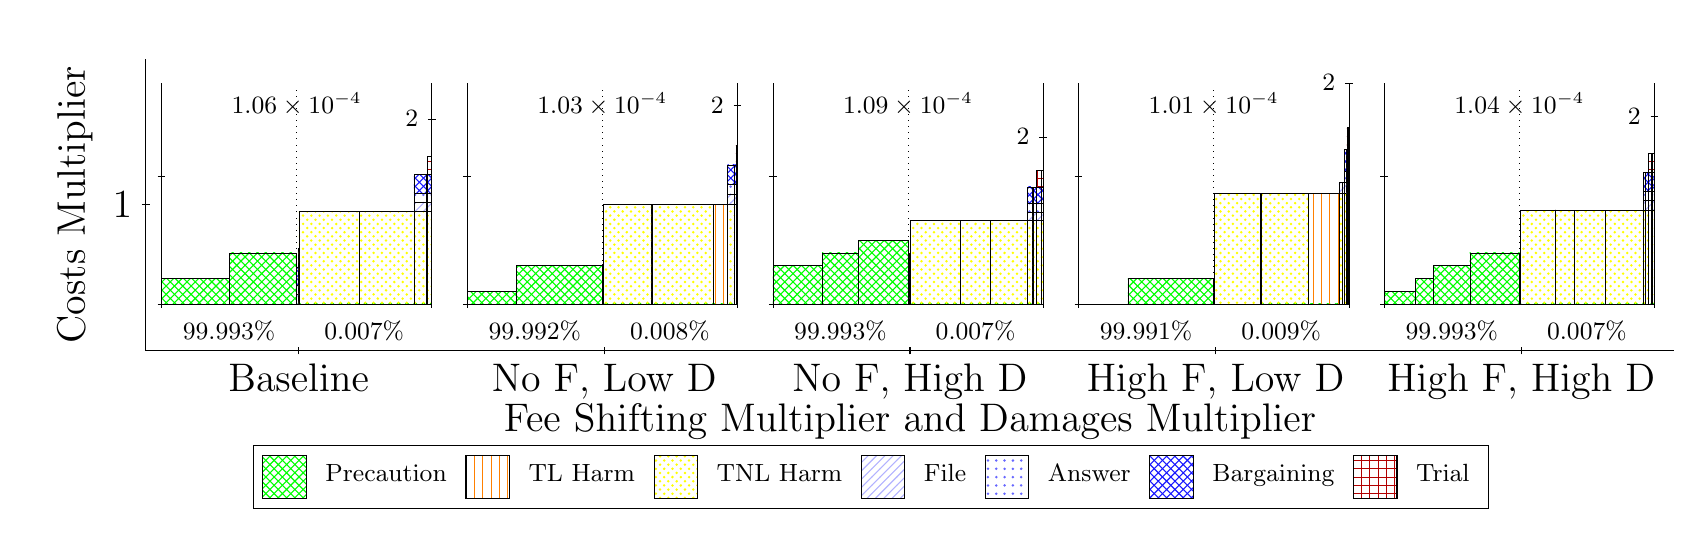
\begin{tikzpicture}
\clip(-0.5,-1.1) rectangle +(20.91,6.2);
\draw[black] (1,1) -- (1,4.7);
\node[rotate=90, fontscale=2, anchor=center] at (0.1, 2.85) {Costs Multiplier};
\draw[black] (0.95,2.85) -- (1.05,2.85);
\node[fontscale=2, anchor=east] at (0.95, 2.85) {1};

\draw[black] (1,1) -- (20.41,1);
\node[fontscale=2, anchor=center] at (10.705, 0.1) {Fee Shifting Multiplier and Damages Multiplier};
\draw[black] (2.941,0.95) -- (2.941,1.05);
\node[fontscale=2, anchor=north] at (2.941, 0.95) {Baseline};
\draw[black] (6.823,0.95) -- (6.823,1.05);
\node[fontscale=2, anchor=north] at (6.823, 0.95) {No F, Low D};
\draw[black] (10.705,0.95) -- (10.705,1.05);
\node[fontscale=2, anchor=north] at (10.705, 0.95) {No F, High D};
\draw[black] (14.587,0.95) -- (14.587,1.05);
\node[fontscale=2, anchor=north] at (14.587, 0.95) {High F, Low D};
\draw[black] (18.469,0.95) -- (18.469,1.05);
\node[fontscale=2, anchor=north] at (18.469, 0.95) {High F, High D};


\draw[pattern=crosshatch, pattern color=green,draw=black,very thin] (1.2,1.592) rectangle (2.058,1.916);
\draw[pattern=crosshatch, pattern color=green,draw=black,very thin] (2.058,1.592) rectangle (2.916,2.24);
\draw[pattern=crosshatch, pattern color=green,draw=black,very thin] (2.916,1.592) rectangle (2.9373,1.592);
\draw[pattern=north east lines, pattern color=blue!30,draw=black,very thin] (2.916,1.592) rectangle (2.9373,1.7095);
\draw[pattern=dots,  pattern color=blue!60,draw=black,very thin] (2.916,1.7095) rectangle (2.9373,1.827);
\draw[pattern=crosshatch,      pattern color=blue!90,draw=black,very thin] (2.916,1.827) rectangle (2.9373,2.062);
\draw[pattern=crosshatch, pattern color=green,draw=black,very thin] (2.9373,1.592) rectangle (2.9441,1.592);
\draw[pattern=north east lines, pattern color=blue!30,draw=black,very thin] (2.9373,1.592) rectangle (2.9441,1.7095);
\draw[pattern=dots,  pattern color=blue!60,draw=black,very thin] (2.9373,1.7095) rectangle (2.9441,1.827);
\draw[pattern=crosshatch,      pattern color=blue!90,draw=black,very thin] (2.9373,1.827) rectangle (2.9441,2.062);
\draw[pattern=grid,            pattern color=red!70!black,draw=black,very thin] (2.9373,2.062) rectangle (2.9441,2.297);
\draw[pattern=crosshatch, pattern color=green,draw=black,very thin] (2.9441,1.592) rectangle (3.7125,1.592);
\draw[pattern=crosshatch dots, pattern color=yellow,draw=black,very thin] (2.9441,1.592) rectangle (3.7125,2.767);
\draw[pattern=crosshatch, pattern color=green,draw=black,very thin] (3.7125,1.592) rectangle (3.7131,1.592);
\draw[pattern=vertical lines, pattern color=orange,draw=black,very thin] (3.7125,1.592) rectangle (3.7131,2.767);
\draw[pattern=crosshatch, pattern color=green,draw=black,very thin] (3.7131,1.592) rectangle (4.4059,1.592);
\draw[pattern=crosshatch dots, pattern color=yellow,draw=black,very thin] (3.7131,1.592) rectangle (4.4059,2.767);
\draw[pattern=crosshatch, pattern color=green,draw=black,very thin] (4.4059,1.592) rectangle (4.557,1.592);
\draw[pattern=crosshatch dots, pattern color=yellow,draw=black,very thin] (4.4059,1.592) rectangle (4.557,2.767);
\draw[pattern=north east lines, pattern color=blue!30,draw=black,very thin] (4.4059,2.767) rectangle (4.557,2.8845);
\draw[pattern=dots,  pattern color=blue!60,draw=black,very thin] (4.4059,2.8845) rectangle (4.557,3.002);
\draw[pattern=crosshatch,      pattern color=blue!90,draw=black,very thin] (4.4059,3.002) rectangle (4.557,3.237);
\draw[pattern=crosshatch, pattern color=green,draw=black,very thin] (4.557,1.592) rectangle (4.5755,1.592);
\draw[pattern=vertical lines, pattern color=orange,draw=black,very thin] (4.557,1.592) rectangle (4.5755,2.767);
\draw[pattern=north east lines, pattern color=blue!30,draw=black,very thin] (4.557,2.767) rectangle (4.5755,2.8845);
\draw[pattern=dots,  pattern color=blue!60,draw=black,very thin] (4.557,2.8845) rectangle (4.5755,3.002);
\draw[pattern=crosshatch,      pattern color=blue!90,draw=black,very thin] (4.557,3.002) rectangle (4.5755,3.237);
\draw[pattern=crosshatch, pattern color=green,draw=black,very thin] (4.5755,1.592) rectangle (4.6315,1.592);
\draw[pattern=crosshatch dots, pattern color=yellow,draw=black,very thin] (4.5755,1.592) rectangle (4.6315,2.767);
\draw[pattern=north east lines, pattern color=blue!30,draw=black,very thin] (4.5755,2.767) rectangle (4.6315,2.8845);
\draw[pattern=dots,  pattern color=blue!60,draw=black,very thin] (4.5755,2.8845) rectangle (4.6315,3.002);
\draw[pattern=crosshatch,      pattern color=blue!90,draw=black,very thin] (4.5755,3.002) rectangle (4.6315,3.237);
\draw[pattern=grid,            pattern color=red!70!black,draw=black,very thin] (4.5755,3.237) rectangle (4.6315,3.472);
\draw[pattern=crosshatch, pattern color=green,draw=black,very thin] (4.6315,1.592) rectangle (4.632,1.592);
\draw[pattern=vertical lines, pattern color=orange,draw=black,very thin] (4.6315,1.592) rectangle (4.632,2.767);
\draw[pattern=north east lines, pattern color=blue!30,draw=black,very thin] (4.6315,2.767) rectangle (4.632,2.8845);
\draw[pattern=dots,  pattern color=blue!60,draw=black,very thin] (4.6315,2.8845) rectangle (4.632,3.002);
\draw[pattern=crosshatch,      pattern color=blue!90,draw=black,very thin] (4.6315,3.002) rectangle (4.632,3.237);
\draw[pattern=grid,            pattern color=red!70!black,draw=black,very thin] (4.6315,3.237) rectangle (4.632,3.472);
\node[font=\small,text=black,anchor=north] at (2.916, 4.4) {$1.06\times 10^{-4}$};
\draw[black,very thin] (1.2,1.592) -- (1.2,4.4);
\draw[black,very thin] (1.15,1.592) -- (1.25,1.592);
\node[font=\small,text=black, anchor=west] at (1.15, 1.592) {};
\draw[black,very thin] (1.15,3.2119) -- (1.25,3.2119);
\node[font=\small,text=black, anchor=west] at (1.15, 3.2119) {};

\draw[black,dotted,very thin] (2.916,1.6762) -- (2.916,4.3158);
\draw[black,very thin] (4.632,1.592) -- (4.632,4.4);
\draw[black,very thin] (4.582,3.942) -- (4.682,3.942);
\node[font=\small,text=black, anchor=east] at (4.582, 3.942) {\contour{white}{2}};

\draw[black,very thin] (1.2,1.592) -- (4.632,1.592);
\draw[black,very thin] (1.2,1.542) -- (1.2,1.642);
\node[font=\small,text=black, anchor=north] at (1.2, 1.542) {};
\draw[black,very thin] (4.632,1.542) -- (4.632,1.642);
\node[font=\small,text=black, anchor=north] at (4.632, 1.542) {};

\node[font=\small,text=black,anchor=south] at (2.058, 0.992) {99.993\%};
\node[font=\small,text=black,anchor=south] at (3.774, 0.992) {0.007\%};

\draw[pattern=crosshatch, pattern color=green,draw=black,very thin] (5.082,1.592) rectangle (5.7085,1.754);
\draw[pattern=crosshatch, pattern color=green,draw=black,very thin] (5.7085,1.592) rectangle (6.798,2.078);
\draw[pattern=crosshatch, pattern color=green,draw=black,very thin] (6.798,1.592) rectangle (6.8099,1.592);
\draw[pattern=north east lines, pattern color=blue!30,draw=black,very thin] (6.798,1.592) rectangle (6.8099,1.7181);
\draw[pattern=dots,  pattern color=blue!60,draw=black,very thin] (6.798,1.7181) rectangle (6.8099,1.8442);
\draw[pattern=crosshatch,      pattern color=blue!90,draw=black,very thin] (6.798,1.8442) rectangle (6.8099,2.0963);
\draw[pattern=crosshatch, pattern color=green,draw=black,very thin] (6.8099,1.592) rectangle (6.812,1.592);
\draw[pattern=north east lines, pattern color=blue!30,draw=black,very thin] (6.8099,1.592) rectangle (6.812,1.7181);
\draw[pattern=dots,  pattern color=blue!60,draw=black,very thin] (6.8099,1.7181) rectangle (6.812,1.8442);
\draw[pattern=crosshatch,      pattern color=blue!90,draw=black,very thin] (6.8099,1.8442) rectangle (6.812,2.0963);
\draw[pattern=grid,            pattern color=red!70!black,draw=black,very thin] (6.8099,2.0963) rectangle (6.812,2.3484);
\draw[pattern=crosshatch, pattern color=green,draw=black,very thin] (6.812,1.592) rectangle (7.4254,1.592);
\draw[pattern=crosshatch dots, pattern color=yellow,draw=black,very thin] (6.812,1.592) rectangle (7.4254,2.8527);
\draw[pattern=crosshatch, pattern color=green,draw=black,very thin] (7.4254,1.592) rectangle (7.427,1.592);
\draw[pattern=vertical lines, pattern color=orange,draw=black,very thin] (7.4254,1.592) rectangle (7.427,2.8527);
\draw[pattern=crosshatch, pattern color=green,draw=black,very thin] (7.427,1.592) rectangle (8.2015,1.592);
\draw[pattern=crosshatch dots, pattern color=yellow,draw=black,very thin] (7.427,1.592) rectangle (8.2015,2.8527);
\draw[pattern=crosshatch, pattern color=green,draw=black,very thin] (8.2015,1.592) rectangle (8.3877,1.592);
\draw[pattern=vertical lines, pattern color=orange,draw=black,very thin] (8.2015,1.592) rectangle (8.3877,2.8527);
\draw[pattern=crosshatch, pattern color=green,draw=black,very thin] (8.3877,1.592) rectangle (8.4796,1.592);
\draw[pattern=crosshatch dots, pattern color=yellow,draw=black,very thin] (8.3877,1.592) rectangle (8.4796,2.8527);
\draw[pattern=north east lines, pattern color=blue!30,draw=black,very thin] (8.3877,2.8527) rectangle (8.4796,2.9788);
\draw[pattern=dots,  pattern color=blue!60,draw=black,very thin] (8.3877,2.9788) rectangle (8.4796,3.1049);
\draw[pattern=crosshatch,      pattern color=blue!90,draw=black,very thin] (8.3877,3.1049) rectangle (8.4796,3.357);
\draw[pattern=crosshatch, pattern color=green,draw=black,very thin] (8.4796,1.592) rectangle (8.4948,1.592);
\draw[pattern=vertical lines, pattern color=orange,draw=black,very thin] (8.4796,1.592) rectangle (8.4948,2.8527);
\draw[pattern=north east lines, pattern color=blue!30,draw=black,very thin] (8.4796,2.8527) rectangle (8.4948,2.9788);
\draw[pattern=dots,  pattern color=blue!60,draw=black,very thin] (8.4796,2.9788) rectangle (8.4948,3.1049);
\draw[pattern=crosshatch,      pattern color=blue!90,draw=black,very thin] (8.4796,3.1049) rectangle (8.4948,3.357);
\draw[pattern=crosshatch, pattern color=green,draw=black,very thin] (8.4948,1.592) rectangle (8.5136,1.592);
\draw[pattern=crosshatch dots, pattern color=yellow,draw=black,very thin] (8.4948,1.592) rectangle (8.5136,2.8527);
\draw[pattern=north east lines, pattern color=blue!30,draw=black,very thin] (8.4948,2.8527) rectangle (8.5136,2.9788);
\draw[pattern=dots,  pattern color=blue!60,draw=black,very thin] (8.4948,2.9788) rectangle (8.5136,3.1049);
\draw[pattern=crosshatch,      pattern color=blue!90,draw=black,very thin] (8.4948,3.1049) rectangle (8.5136,3.357);
\draw[pattern=grid,            pattern color=red!70!black,draw=black,very thin] (8.4948,3.357) rectangle (8.5136,3.6091);
\draw[pattern=crosshatch, pattern color=green,draw=black,very thin] (8.5136,1.592) rectangle (8.514,1.592);
\draw[pattern=vertical lines, pattern color=orange,draw=black,very thin] (8.5136,1.592) rectangle (8.514,2.8527);
\draw[pattern=north east lines, pattern color=blue!30,draw=black,very thin] (8.5136,2.8527) rectangle (8.514,2.9788);
\draw[pattern=dots,  pattern color=blue!60,draw=black,very thin] (8.5136,2.9788) rectangle (8.514,3.1049);
\draw[pattern=crosshatch,      pattern color=blue!90,draw=black,very thin] (8.5136,3.1049) rectangle (8.514,3.357);
\draw[pattern=grid,            pattern color=red!70!black,draw=black,very thin] (8.5136,3.357) rectangle (8.514,3.6091);
\node[font=\small,text=black,anchor=north] at (6.798, 4.4) {$1.03\times 10^{-4}$};
\draw[black,very thin] (5.082,1.592) -- (5.082,4.4);
\draw[black,very thin] (5.032,1.592) -- (5.132,1.592);
\node[font=\small,text=black, anchor=west] at (5.032, 1.592) {};
\draw[black,very thin] (5.032,3.2119) -- (5.132,3.2119);
\node[font=\small,text=black, anchor=west] at (5.032, 3.2119) {};

\draw[black,dotted,very thin] (6.798,1.6762) -- (6.798,4.3158);
\draw[black,very thin] (8.514,1.592) -- (8.514,4.4);
\draw[black,very thin] (8.464,4.1134) -- (8.564,4.1134);
\node[font=\small,text=black, anchor=east] at (8.464, 4.1134) {\contour{white}{2}};

\draw[black,very thin] (5.082,1.592) -- (8.514,1.592);
\draw[black,very thin] (5.082,1.542) -- (5.082,1.642);
\node[font=\small,text=black, anchor=north] at (5.082, 1.542) {};
\draw[black,very thin] (8.514,1.542) -- (8.514,1.642);
\node[font=\small,text=black, anchor=north] at (8.514, 1.542) {};

\node[font=\small,text=black,anchor=south] at (5.94, 0.992) {99.992\%};
\node[font=\small,text=black,anchor=south] at (7.656, 0.992) {0.008\%};

\draw[pattern=crosshatch, pattern color=green,draw=black,very thin] (8.964,1.592) rectangle (9.5905,2.078);
\draw[pattern=crosshatch, pattern color=green,draw=black,very thin] (9.5905,1.592) rectangle (10.053,2.24);
\draw[pattern=crosshatch, pattern color=green,draw=black,very thin] (10.053,1.592) rectangle (10.68,2.402);
\draw[pattern=crosshatch, pattern color=green,draw=black,very thin] (10.68,1.592) rectangle (10.689,1.592);
\draw[pattern=north east lines, pattern color=blue!30,draw=black,very thin] (10.68,1.592) rectangle (10.689,1.6981);
\draw[pattern=dots,  pattern color=blue!60,draw=black,very thin] (10.68,1.6981) rectangle (10.689,1.8042);
\draw[pattern=crosshatch,      pattern color=blue!90,draw=black,very thin] (10.68,1.8042) rectangle (10.689,2.0164);
\draw[pattern=crosshatch, pattern color=green,draw=black,very thin] (10.689,1.592) rectangle (10.697,1.592);
\draw[pattern=north east lines, pattern color=blue!30,draw=black,very thin] (10.689,1.592) rectangle (10.697,1.6981);
\draw[pattern=dots,  pattern color=blue!60,draw=black,very thin] (10.689,1.6981) rectangle (10.697,1.8042);
\draw[pattern=crosshatch,      pattern color=blue!90,draw=black,very thin] (10.689,1.8042) rectangle (10.697,2.0165);
\draw[pattern=crosshatch, pattern color=green,draw=black,very thin] (10.697,1.592) rectangle (10.705,1.592);
\draw[pattern=north east lines, pattern color=blue!30,draw=black,very thin] (10.697,1.592) rectangle (10.705,1.6981);
\draw[pattern=dots,  pattern color=blue!60,draw=black,very thin] (10.697,1.6981) rectangle (10.705,1.8042);
\draw[pattern=crosshatch,      pattern color=blue!90,draw=black,very thin] (10.697,1.8042) rectangle (10.705,2.0164);
\draw[pattern=grid,            pattern color=red!70!black,draw=black,very thin] (10.697,2.0164) rectangle (10.705,2.2286);
\draw[pattern=crosshatch, pattern color=green,draw=black,very thin] (10.705,1.592) rectangle (10.71,1.592);
\draw[pattern=north east lines, pattern color=blue!30,draw=black,very thin] (10.705,1.592) rectangle (10.71,1.6981);
\draw[pattern=dots,  pattern color=blue!60,draw=black,very thin] (10.705,1.6981) rectangle (10.71,1.8042);
\draw[pattern=crosshatch,      pattern color=blue!90,draw=black,very thin] (10.705,1.8042) rectangle (10.71,2.0165);
\draw[pattern=grid,            pattern color=red!70!black,draw=black,very thin] (10.705,2.0165) rectangle (10.71,2.2287);
\draw[pattern=crosshatch, pattern color=green,draw=black,very thin] (10.71,1.592) rectangle (11.342,1.592);
\draw[pattern=crosshatch dots, pattern color=yellow,draw=black,very thin] (10.71,1.592) rectangle (11.342,2.6531);
\draw[pattern=crosshatch, pattern color=green,draw=black,very thin] (11.342,1.592) rectangle (11.728,1.592);
\draw[pattern=crosshatch dots, pattern color=yellow,draw=black,very thin] (11.342,1.592) rectangle (11.728,2.6531);
\draw[pattern=crosshatch, pattern color=green,draw=black,very thin] (11.728,1.592) rectangle (12.199,1.5921);
\draw[pattern=crosshatch dots, pattern color=yellow,draw=black,very thin] (11.728,1.5921) rectangle (12.199,2.6531);
\draw[pattern=crosshatch, pattern color=green,draw=black,very thin] (12.199,1.592) rectangle (12.264,1.592);
\draw[pattern=crosshatch dots, pattern color=yellow,draw=black,very thin] (12.199,1.592) rectangle (12.264,2.6531);
\draw[pattern=north east lines, pattern color=blue!30,draw=black,very thin] (12.199,2.6531) rectangle (12.264,2.7592);
\draw[pattern=dots,  pattern color=blue!60,draw=black,very thin] (12.199,2.7592) rectangle (12.264,2.8653);
\draw[pattern=crosshatch,      pattern color=blue!90,draw=black,very thin] (12.199,2.8653) rectangle (12.264,3.0775);
\draw[pattern=crosshatch, pattern color=green,draw=black,very thin] (12.264,1.592) rectangle (12.265,1.592);
\draw[pattern=vertical lines, pattern color=orange,draw=black,very thin] (12.264,1.592) rectangle (12.265,2.6531);
\draw[pattern=north east lines, pattern color=blue!30,draw=black,very thin] (12.264,2.6531) rectangle (12.265,2.7592);
\draw[pattern=dots,  pattern color=blue!60,draw=black,very thin] (12.264,2.7592) rectangle (12.265,2.8653);
\draw[pattern=crosshatch,      pattern color=blue!90,draw=black,very thin] (12.264,2.8653) rectangle (12.265,3.0775);
\draw[pattern=crosshatch, pattern color=green,draw=black,very thin] (12.265,1.592) rectangle (12.312,1.592);
\draw[pattern=crosshatch dots, pattern color=yellow,draw=black,very thin] (12.265,1.592) rectangle (12.312,2.6531);
\draw[pattern=north east lines, pattern color=blue!30,draw=black,very thin] (12.265,2.6531) rectangle (12.312,2.7592);
\draw[pattern=dots,  pattern color=blue!60,draw=black,very thin] (12.265,2.7592) rectangle (12.312,2.8653);
\draw[pattern=crosshatch,      pattern color=blue!90,draw=black,very thin] (12.265,2.8653) rectangle (12.312,3.0775);
\draw[pattern=crosshatch, pattern color=green,draw=black,very thin] (12.312,1.592) rectangle (12.369,1.592);
\draw[pattern=crosshatch dots, pattern color=yellow,draw=black,very thin] (12.312,1.592) rectangle (12.369,2.6531);
\draw[pattern=north east lines, pattern color=blue!30,draw=black,very thin] (12.312,2.6531) rectangle (12.369,2.7592);
\draw[pattern=dots,  pattern color=blue!60,draw=black,very thin] (12.312,2.7592) rectangle (12.369,2.8653);
\draw[pattern=crosshatch,      pattern color=blue!90,draw=black,very thin] (12.312,2.8653) rectangle (12.369,3.0775);
\draw[pattern=grid,            pattern color=red!70!black,draw=black,very thin] (12.312,3.0775) rectangle (12.369,3.2897);
\draw[pattern=crosshatch, pattern color=green,draw=black,very thin] (12.369,1.592) rectangle (12.396,1.592);
\draw[pattern=crosshatch dots, pattern color=yellow,draw=black,very thin] (12.369,1.592) rectangle (12.396,2.6531);
\draw[pattern=north east lines, pattern color=blue!30,draw=black,very thin] (12.369,2.6531) rectangle (12.396,2.7592);
\draw[pattern=dots,  pattern color=blue!60,draw=black,very thin] (12.369,2.7592) rectangle (12.396,2.8653);
\draw[pattern=crosshatch,      pattern color=blue!90,draw=black,very thin] (12.369,2.8653) rectangle (12.396,3.0775);
\draw[pattern=grid,            pattern color=red!70!black,draw=black,very thin] (12.369,3.0775) rectangle (12.396,3.2897);
\node[font=\small,text=black,anchor=north] at (10.68, 4.4) {$1.09\times 10^{-4}$};
\draw[black,very thin] (8.964,1.592) -- (8.964,4.4);
\draw[black,very thin] (8.914,1.592) -- (9.014,1.592);
\node[font=\small,text=black, anchor=west] at (8.914, 1.592) {};
\draw[black,very thin] (8.914,3.2119) -- (9.014,3.2119);
\node[font=\small,text=black, anchor=west] at (8.914, 3.2119) {};

\draw[black,dotted,very thin] (10.68,1.6762) -- (10.68,4.3158);
\draw[black,very thin] (12.396,1.592) -- (12.396,4.4);
\draw[black,very thin] (12.346,3.7141) -- (12.446,3.7141);
\node[font=\small,text=black, anchor=east] at (12.346, 3.7141) {\contour{white}{2}};

\draw[black,very thin] (8.964,1.592) -- (12.396,1.592);
\draw[black,very thin] (8.964,1.542) -- (8.964,1.642);
\node[font=\small,text=black, anchor=north] at (8.964, 1.542) {};
\draw[black,very thin] (12.396,1.542) -- (12.396,1.642);
\node[font=\small,text=black, anchor=north] at (12.396, 1.542) {};

\node[font=\small,text=black,anchor=south] at (9.822, 0.992) {99.993\%};
\node[font=\small,text=black,anchor=south] at (11.538, 0.992) {0.007\%};

\draw[pattern=crosshatch, pattern color=green,draw=black,very thin] (13.473,1.592) rectangle (14.562,1.916);
\draw[pattern=north east lines, pattern color=blue!30,draw=black,very thin] (14.562,1.592) rectangle (14.569,1.7324);
\draw[pattern=north east lines, pattern color=blue!30,draw=black,very thin] (14.569,1.592) rectangle (14.572,1.7324);
\draw[pattern=dots,  pattern color=blue!60,draw=black,very thin] (14.569,1.7324) rectangle (14.572,1.8728);
\draw[pattern=crosshatch,      pattern color=blue!90,draw=black,very thin] (14.569,1.8728) rectangle (14.572,2.1536);
\draw[pattern=north east lines, pattern color=blue!30,draw=black,very thin] (14.572,1.592) rectangle (14.575,1.7324);
\draw[pattern=dots,  pattern color=blue!60,draw=black,very thin] (14.572,1.7324) rectangle (14.575,1.8728);
\draw[pattern=crosshatch,      pattern color=blue!90,draw=black,very thin] (14.572,1.8728) rectangle (14.575,2.1536);
\draw[pattern=grid,            pattern color=red!70!black,draw=black,very thin] (14.572,2.1536) rectangle (14.575,2.4344);
\draw[pattern=crosshatch dots, pattern color=yellow,draw=black,very thin] (14.575,1.592) rectangle (15.159,2.996);
\draw[pattern=vertical lines, pattern color=orange,draw=black,very thin] (15.159,1.592) rectangle (15.172,2.996);
\draw[pattern=crosshatch, pattern color=green,draw=black,very thin] (15.172,1.592) rectangle (15.767,1.592);
\draw[pattern=crosshatch dots, pattern color=yellow,draw=black,very thin] (15.172,1.592) rectangle (15.767,2.996);
\draw[pattern=crosshatch, pattern color=green,draw=black,very thin] (15.767,1.592) rectangle (16.152,1.592);
\draw[pattern=vertical lines, pattern color=orange,draw=black,very thin] (15.767,1.592) rectangle (16.152,2.996);
\draw[pattern=crosshatch dots, pattern color=yellow,draw=black,very thin] (16.152,1.592) rectangle (16.19,2.996);
\draw[pattern=north east lines, pattern color=blue!30,draw=black,very thin] (16.152,2.996) rectangle (16.19,3.1364);
\draw[pattern=vertical lines, pattern color=orange,draw=black,very thin] (16.19,1.592) rectangle (16.221,2.996);
\draw[pattern=north east lines, pattern color=blue!30,draw=black,very thin] (16.19,2.996) rectangle (16.221,3.1364);
\draw[pattern=crosshatch dots, pattern color=yellow,draw=black,very thin] (16.221,1.592) rectangle (16.251,2.996);
\draw[pattern=north east lines, pattern color=blue!30,draw=black,very thin] (16.221,2.996) rectangle (16.251,3.1364);
\draw[pattern=dots,  pattern color=blue!60,draw=black,very thin] (16.221,3.1364) rectangle (16.251,3.2768);
\draw[pattern=crosshatch,      pattern color=blue!90,draw=black,very thin] (16.221,3.2768) rectangle (16.251,3.5576);
\draw[pattern=vertical lines, pattern color=orange,draw=black,very thin] (16.251,1.592) rectangle (16.255,2.996);
\draw[pattern=north east lines, pattern color=blue!30,draw=black,very thin] (16.251,2.996) rectangle (16.255,3.1364);
\draw[pattern=dots,  pattern color=blue!60,draw=black,very thin] (16.251,3.1364) rectangle (16.255,3.2768);
\draw[pattern=crosshatch,      pattern color=blue!90,draw=black,very thin] (16.251,3.2768) rectangle (16.255,3.5576);
\draw[pattern=crosshatch dots, pattern color=yellow,draw=black,very thin] (16.255,1.592) rectangle (16.27,2.996);
\draw[pattern=north east lines, pattern color=blue!30,draw=black,very thin] (16.255,2.996) rectangle (16.27,3.1364);
\draw[pattern=dots,  pattern color=blue!60,draw=black,very thin] (16.255,3.1364) rectangle (16.27,3.2768);
\draw[pattern=crosshatch,      pattern color=blue!90,draw=black,very thin] (16.255,3.2768) rectangle (16.27,3.5576);
\draw[pattern=grid,            pattern color=red!70!black,draw=black,very thin] (16.255,3.5576) rectangle (16.27,3.8384);
\draw[pattern=vertical lines, pattern color=orange,draw=black,very thin] (16.27,1.592) rectangle (16.278,2.996);
\draw[pattern=north east lines, pattern color=blue!30,draw=black,very thin] (16.27,2.996) rectangle (16.278,3.1364);
\draw[pattern=dots,  pattern color=blue!60,draw=black,very thin] (16.27,3.1364) rectangle (16.278,3.2768);
\draw[pattern=crosshatch,      pattern color=blue!90,draw=black,very thin] (16.27,3.2768) rectangle (16.278,3.5576);
\draw[pattern=grid,            pattern color=red!70!black,draw=black,very thin] (16.27,3.5576) rectangle (16.278,3.8384);
\node[font=\small,text=black,anchor=north] at (14.562, 4.4) {$1.01\times 10^{-4}$};
\draw[black,very thin] (12.846,1.592) -- (12.846,4.4);
\draw[black,very thin] (12.796,1.592) -- (12.896,1.592);
\node[font=\small,text=black, anchor=west] at (12.796, 1.592) {};
\draw[black,very thin] (12.796,3.2119) -- (12.896,3.2119);
\node[font=\small,text=black, anchor=west] at (12.796, 3.2119) {};

\draw[black,dotted,very thin] (14.562,1.6762) -- (14.562,4.3158);
\draw[black,very thin] (16.278,1.592) -- (16.278,4.4);
\draw[black,very thin] (16.228,4.4) -- (16.328,4.4);
\node[font=\small,text=black, anchor=east] at (16.228, 4.4) {\contour{white}{2}};

\draw[black,very thin] (12.846,1.592) -- (16.278,1.592);
\draw[black,very thin] (12.846,1.542) -- (12.846,1.642);
\node[font=\small,text=black, anchor=north] at (12.846, 1.542) {};
\draw[black,very thin] (16.278,1.542) -- (16.278,1.642);
\node[font=\small,text=black, anchor=north] at (16.278, 1.542) {};

\node[font=\small,text=black,anchor=south] at (13.704, 0.992) {99.991\%};
\node[font=\small,text=black,anchor=south] at (15.42, 0.992) {0.009\%};

\draw[pattern=crosshatch, pattern color=green,draw=black,very thin] (16.728,1.592) rectangle (17.123,1.754);
\draw[pattern=crosshatch, pattern color=green,draw=black,very thin] (17.123,1.592) rectangle (17.355,1.916);
\draw[pattern=crosshatch, pattern color=green,draw=black,very thin] (17.355,1.592) rectangle (17.817,2.078);
\draw[pattern=crosshatch, pattern color=green,draw=black,very thin] (17.817,1.592) rectangle (18.444,2.24);
\draw[pattern=crosshatch, pattern color=green,draw=black,very thin] (18.444,1.592) rectangle (18.447,1.592);
\draw[pattern=north east lines, pattern color=blue!30,draw=black,very thin] (18.444,1.592) rectangle (18.447,1.7113);
\draw[pattern=dots,  pattern color=blue!60,draw=black,very thin] (18.444,1.7113) rectangle (18.447,1.8306);
\draw[pattern=crosshatch,      pattern color=blue!90,draw=black,very thin] (18.444,1.8306) rectangle (18.447,2.0692);
\draw[pattern=crosshatch, pattern color=green,draw=black,very thin] (18.447,1.592) rectangle (18.453,1.592);
\draw[pattern=north east lines, pattern color=blue!30,draw=black,very thin] (18.447,1.592) rectangle (18.453,1.7113);
\draw[pattern=dots,  pattern color=blue!60,draw=black,very thin] (18.447,1.7113) rectangle (18.453,1.8306);
\draw[pattern=crosshatch,      pattern color=blue!90,draw=black,very thin] (18.447,1.8306) rectangle (18.453,2.0692);
\draw[pattern=crosshatch, pattern color=green,draw=black,very thin] (18.453,1.592) rectangle (18.457,1.592);
\draw[pattern=north east lines, pattern color=blue!30,draw=black,very thin] (18.453,1.592) rectangle (18.457,1.7113);
\draw[pattern=dots,  pattern color=blue!60,draw=black,very thin] (18.453,1.7113) rectangle (18.457,1.8306);
\draw[pattern=crosshatch,      pattern color=blue!90,draw=black,very thin] (18.453,1.8306) rectangle (18.457,2.0692);
\draw[pattern=grid,            pattern color=red!70!black,draw=black,very thin] (18.453,2.0692) rectangle (18.457,2.3078);
\draw[pattern=crosshatch, pattern color=green,draw=black,very thin] (18.457,1.592) rectangle (18.459,1.592);
\draw[pattern=north east lines, pattern color=blue!30,draw=black,very thin] (18.457,1.592) rectangle (18.459,1.7113);
\draw[pattern=dots,  pattern color=blue!60,draw=black,very thin] (18.457,1.7113) rectangle (18.459,1.8306);
\draw[pattern=crosshatch,      pattern color=blue!90,draw=black,very thin] (18.457,1.8306) rectangle (18.459,2.0692);
\draw[pattern=grid,            pattern color=red!70!black,draw=black,very thin] (18.457,2.0692) rectangle (18.459,2.3078);
\draw[pattern=crosshatch, pattern color=green,draw=black,very thin] (18.459,1.592) rectangle (18.462,1.592);
\draw[pattern=north east lines, pattern color=blue!30,draw=black,very thin] (18.459,1.592) rectangle (18.462,1.7113);
\draw[pattern=dots,  pattern color=blue!60,draw=black,very thin] (18.459,1.7113) rectangle (18.462,1.8306);
\draw[pattern=crosshatch,      pattern color=blue!90,draw=black,very thin] (18.459,1.8306) rectangle (18.462,2.0692);
\draw[pattern=grid,            pattern color=red!70!black,draw=black,very thin] (18.459,2.0692) rectangle (18.462,2.3078);
\draw[pattern=crosshatch, pattern color=green,draw=black,very thin] (18.462,1.592) rectangle (18.897,1.592);
\draw[pattern=crosshatch dots, pattern color=yellow,draw=black,very thin] (18.462,1.592) rectangle (18.897,2.7849);
\draw[pattern=crosshatch, pattern color=green,draw=black,very thin] (18.897,1.592) rectangle (18.897,1.592);
\draw[pattern=vertical lines, pattern color=orange,draw=black,very thin] (18.897,1.592) rectangle (18.897,2.7849);
\draw[pattern=crosshatch, pattern color=green,draw=black,very thin] (18.897,1.592) rectangle (19.145,1.592);
\draw[pattern=crosshatch dots, pattern color=yellow,draw=black,very thin] (18.897,1.592) rectangle (19.145,2.785);
\draw[pattern=crosshatch, pattern color=green,draw=black,very thin] (19.145,1.592) rectangle (19.146,1.592);
\draw[pattern=vertical lines, pattern color=orange,draw=black,very thin] (19.145,1.592) rectangle (19.146,2.785);
\draw[pattern=crosshatch, pattern color=green,draw=black,very thin] (19.146,1.592) rectangle (19.53,1.592);
\draw[pattern=crosshatch dots, pattern color=yellow,draw=black,very thin] (19.146,1.592) rectangle (19.53,2.785);
\draw[pattern=crosshatch, pattern color=green,draw=black,very thin] (19.53,1.592) rectangle (19.535,1.592);
\draw[pattern=vertical lines, pattern color=orange,draw=black,very thin] (19.53,1.592) rectangle (19.535,2.785);
\draw[pattern=crosshatch, pattern color=green,draw=black,very thin] (19.535,1.592) rectangle (20.02,1.592);
\draw[pattern=crosshatch dots, pattern color=yellow,draw=black,very thin] (19.535,1.592) rectangle (20.02,2.785);
\draw[pattern=crosshatch, pattern color=green,draw=black,very thin] (20.02,1.592) rectangle (20.042,1.592);
\draw[pattern=crosshatch dots, pattern color=yellow,draw=black,very thin] (20.02,1.592) rectangle (20.042,2.7849);
\draw[pattern=north east lines, pattern color=blue!30,draw=black,very thin] (20.02,2.7849) rectangle (20.042,2.9042);
\draw[pattern=dots,  pattern color=blue!60,draw=black,very thin] (20.02,2.9042) rectangle (20.042,3.0235);
\draw[pattern=crosshatch,      pattern color=blue!90,draw=black,very thin] (20.02,3.0235) rectangle (20.042,3.2621);
\draw[pattern=crosshatch, pattern color=green,draw=black,very thin] (20.042,1.592) rectangle (20.043,1.592);
\draw[pattern=vertical lines, pattern color=orange,draw=black,very thin] (20.042,1.592) rectangle (20.043,2.7849);
\draw[pattern=north east lines, pattern color=blue!30,draw=black,very thin] (20.042,2.7849) rectangle (20.043,2.9042);
\draw[pattern=dots,  pattern color=blue!60,draw=black,very thin] (20.042,2.9042) rectangle (20.043,3.0235);
\draw[pattern=crosshatch,      pattern color=blue!90,draw=black,very thin] (20.042,3.0235) rectangle (20.043,3.2621);
\draw[pattern=crosshatch, pattern color=green,draw=black,very thin] (20.043,1.592) rectangle (20.076,1.592);
\draw[pattern=crosshatch dots, pattern color=yellow,draw=black,very thin] (20.043,1.592) rectangle (20.076,2.785);
\draw[pattern=north east lines, pattern color=blue!30,draw=black,very thin] (20.043,2.785) rectangle (20.076,2.9043);
\draw[pattern=dots,  pattern color=blue!60,draw=black,very thin] (20.043,2.9043) rectangle (20.076,3.0236);
\draw[pattern=crosshatch,      pattern color=blue!90,draw=black,very thin] (20.043,3.0236) rectangle (20.076,3.2621);
\draw[pattern=crosshatch, pattern color=green,draw=black,very thin] (20.076,1.592) rectangle (20.085,1.592);
\draw[pattern=vertical lines, pattern color=orange,draw=black,very thin] (20.076,1.592) rectangle (20.085,2.785);
\draw[pattern=north east lines, pattern color=blue!30,draw=black,very thin] (20.076,2.785) rectangle (20.085,2.9043);
\draw[pattern=dots,  pattern color=blue!60,draw=black,very thin] (20.076,2.9043) rectangle (20.085,3.0236);
\draw[pattern=crosshatch,      pattern color=blue!90,draw=black,very thin] (20.076,3.0236) rectangle (20.085,3.2621);
\draw[pattern=crosshatch, pattern color=green,draw=black,very thin] (20.085,1.592) rectangle (20.12,1.592);
\draw[pattern=crosshatch dots, pattern color=yellow,draw=black,very thin] (20.085,1.592) rectangle (20.12,2.7849);
\draw[pattern=north east lines, pattern color=blue!30,draw=black,very thin] (20.085,2.7849) rectangle (20.12,2.9042);
\draw[pattern=dots,  pattern color=blue!60,draw=black,very thin] (20.085,2.9042) rectangle (20.12,3.0235);
\draw[pattern=crosshatch,      pattern color=blue!90,draw=black,very thin] (20.085,3.0235) rectangle (20.12,3.2621);
\draw[pattern=grid,            pattern color=red!70!black,draw=black,very thin] (20.085,3.2621) rectangle (20.12,3.5007);
\draw[pattern=crosshatch, pattern color=green,draw=black,very thin] (20.12,1.592) rectangle (20.123,1.592);
\draw[pattern=vertical lines, pattern color=orange,draw=black,very thin] (20.12,1.592) rectangle (20.123,2.7849);
\draw[pattern=north east lines, pattern color=blue!30,draw=black,very thin] (20.12,2.7849) rectangle (20.123,2.9042);
\draw[pattern=dots,  pattern color=blue!60,draw=black,very thin] (20.12,2.9042) rectangle (20.123,3.0235);
\draw[pattern=crosshatch,      pattern color=blue!90,draw=black,very thin] (20.12,3.0235) rectangle (20.123,3.2621);
\draw[pattern=grid,            pattern color=red!70!black,draw=black,very thin] (20.12,3.2621) rectangle (20.123,3.5007);
\draw[pattern=crosshatch, pattern color=green,draw=black,very thin] (20.123,1.592) rectangle (20.135,1.592);
\draw[pattern=crosshatch dots, pattern color=yellow,draw=black,very thin] (20.123,1.592) rectangle (20.135,2.785);
\draw[pattern=north east lines, pattern color=blue!30,draw=black,very thin] (20.123,2.785) rectangle (20.135,2.9042);
\draw[pattern=dots,  pattern color=blue!60,draw=black,very thin] (20.123,2.9042) rectangle (20.135,3.0235);
\draw[pattern=crosshatch,      pattern color=blue!90,draw=black,very thin] (20.123,3.0235) rectangle (20.135,3.2621);
\draw[pattern=grid,            pattern color=red!70!black,draw=black,very thin] (20.123,3.2621) rectangle (20.135,3.5007);
\draw[pattern=crosshatch, pattern color=green,draw=black,very thin] (20.135,1.592) rectangle (20.137,1.592);
\draw[pattern=vertical lines, pattern color=orange,draw=black,very thin] (20.135,1.592) rectangle (20.137,2.785);
\draw[pattern=north east lines, pattern color=blue!30,draw=black,very thin] (20.135,2.785) rectangle (20.137,2.9042);
\draw[pattern=dots,  pattern color=blue!60,draw=black,very thin] (20.135,2.9042) rectangle (20.137,3.0235);
\draw[pattern=crosshatch,      pattern color=blue!90,draw=black,very thin] (20.135,3.0235) rectangle (20.137,3.2621);
\draw[pattern=grid,            pattern color=red!70!black,draw=black,very thin] (20.135,3.2621) rectangle (20.137,3.5007);
\draw[pattern=crosshatch, pattern color=green,draw=black,very thin] (20.137,1.592) rectangle (20.158,1.592);
\draw[pattern=crosshatch dots, pattern color=yellow,draw=black,very thin] (20.137,1.592) rectangle (20.158,2.785);
\draw[pattern=north east lines, pattern color=blue!30,draw=black,very thin] (20.137,2.785) rectangle (20.158,2.9043);
\draw[pattern=dots,  pattern color=blue!60,draw=black,very thin] (20.137,2.9043) rectangle (20.158,3.0236);
\draw[pattern=crosshatch,      pattern color=blue!90,draw=black,very thin] (20.137,3.0236) rectangle (20.158,3.2621);
\draw[pattern=grid,            pattern color=red!70!black,draw=black,very thin] (20.137,3.2621) rectangle (20.158,3.5007);
\draw[pattern=crosshatch, pattern color=green,draw=black,very thin] (20.158,1.592) rectangle (20.16,1.592);
\draw[pattern=vertical lines, pattern color=orange,draw=black,very thin] (20.158,1.592) rectangle (20.16,2.785);
\draw[pattern=north east lines, pattern color=blue!30,draw=black,very thin] (20.158,2.785) rectangle (20.16,2.9043);
\draw[pattern=dots,  pattern color=blue!60,draw=black,very thin] (20.158,2.9043) rectangle (20.16,3.0236);
\draw[pattern=crosshatch,      pattern color=blue!90,draw=black,very thin] (20.158,3.0236) rectangle (20.16,3.2621);
\draw[pattern=grid,            pattern color=red!70!black,draw=black,very thin] (20.158,3.2621) rectangle (20.16,3.5007);
\node[font=\small,text=black,anchor=north] at (18.444, 4.4) {$1.04\times 10^{-4}$};
\draw[black,very thin] (16.728,1.592) -- (16.728,4.4);
\draw[black,very thin] (16.678,1.592) -- (16.778,1.592);
\node[font=\small,text=black, anchor=west] at (16.678, 1.592) {};
\draw[black,very thin] (16.678,3.2119) -- (16.778,3.2119);
\node[font=\small,text=black, anchor=west] at (16.678, 3.2119) {};

\draw[black,dotted,very thin] (18.444,1.6762) -- (18.444,4.3158);
\draw[black,very thin] (20.16,1.592) -- (20.16,4.4);
\draw[black,very thin] (20.11,3.9779) -- (20.21,3.9779);
\node[font=\small,text=black, anchor=east] at (20.11, 3.9779) {\contour{white}{2}};

\draw[black,very thin] (16.728,1.592) -- (20.16,1.592);
\draw[black,very thin] (16.728,1.542) -- (16.728,1.642);
\node[font=\small,text=black, anchor=north] at (16.728, 1.542) {};
\draw[black,very thin] (20.16,1.542) -- (20.16,1.642);
\node[font=\small,text=black, anchor=north] at (20.16, 1.542) {};

\node[font=\small,text=black,anchor=south] at (17.586, 0.992) {99.993\%};
\node[font=\small,text=black,anchor=south] at (19.302, 0.992) {0.007\%};

\coordinate (LegendAnchor) at (10.205000000000002,0);
\begin{scope}[align=center]
\matrix[scale=0.6,draw=black,below=0.2cm of LegendAnchor,nodes={draw},column sep=0.12cm]{
\node[rectangle,draw,minimum width=0.55cm,minimum height=0.55cm,pattern=crosshatch, pattern color=green]{}; &
        \node[draw=none,font=\small]{Precaution}; &
\node[rectangle,draw,minimum width=0.55cm,minimum height=0.55cm,pattern=vertical lines, pattern color=orange]{}; &
        \node[draw=none,font=\small]{TL Harm}; &
\node[rectangle,draw,minimum width=0.55cm,minimum height=0.55cm,pattern=crosshatch dots, pattern color=yellow]{}; &
        \node[draw=none,font=\small]{TNL Harm}; &
\node[rectangle,draw,minimum width=0.55cm,minimum height=0.55cm,pattern=north east lines, pattern color=blue!30]{}; &
        \node[draw=none,font=\small]{File}; &
\node[rectangle,draw,minimum width=0.55cm,minimum height=0.55cm,pattern=dots, pattern color=blue!60]{}; &
        \node[draw=none,font=\small]{Answer}; &
\node[rectangle,draw,minimum width=0.55cm,minimum height=0.55cm,pattern=crosshatch, pattern color=blue!90]{}; &
        \node[draw=none,font=\small]{Bargaining}; &
\node[rectangle,draw,minimum width=0.55cm,minimum height=0.55cm,pattern=grid, pattern color=red!70!black]{}; &
        \node[draw=none,font=\small]{Trial}; \\
};\end{scope}

\end{tikzpicture}
\end{document}